% !TEX program = lualatex
% Generated by new_lecture_note.sh
\documentclass[11pt]{article}

\usepackage{fontspec}
\usepackage{microtype}
\usepackage{mathtools,amssymb,amsfonts,amsthm,bm}
\usepackage{enumitem}
\usepackage{spalign}
\usepackage{booktabs,array,xcolor}
\usepackage{tikz}
\usetikzlibrary{arrows.meta}
\usepackage{geometry,fancyhdr,setspace}
\usepackage[hidelinks]{hyperref}
\usepackage[nameinlink,noabbrev]{cleveref}

\geometry{margin=1in,headheight=15pt}
\setstretch{1.12}
\setlength{\parindent}{0pt}
\setlength{\parskip}{0.55em plus 0.12em minus 0.08em}
\setlength{\abovedisplayskip}{0.8em plus 0.2em minus 0.1em}
\setlength{\belowdisplayskip}{0.8em plus 0.2em minus 0.1em}
\allowdisplaybreaks[3]
\setlist{leftmargin=*,topsep=0.35em,itemsep=0.15em,parsep=0pt}

% ---------- Metadata ----------
\newcommand{\studentname}{Keshav Ramamurthy}
\newcommand{\coursename}{Math 118}
\newcommand{\courselongname}{Fourier Analysis}
\newcommand{\lecturenumber}{03}
\newcommand{\lecturetitle}{Lecture 03}
\newcommand{\lecturedate}{\today}

% ---------- Reusable notation ----------
\newcommand{\N}{\mathbb{N}}
\newcommand{\Z}{\mathbb{Z}}
\newcommand{\Q}{\mathbb{Q}}
\newcommand{\R}{\mathbb{R}}
\newcommand{\C}{\mathbb{C}}
\newcommand{\F}{\mathbb{F}}
\newcommand{\K}{\mathbb{K}}
\newcommand{\E}{\mathbb{E}}
\newcommand{\Prob}{\mathbb{P}}
\newcommand{\1}{\mathbf{1}}
\newcommand{\eps}{\varepsilon}
\newcommand{\dd}{\,\mathrm{d}}
\newcommand{\abs}[1]{\left\lvert#1\right\rvert}
\newcommand{\norm}[1]{\left\lVert#1\right\rVert}
\newcommand{\ip}[2]{\left\langle#1,#2\right\rangle}
\newcommand{\set}[1]{\left\{#1\right\}}
\newcommand{\given}{\,\middle\vert\,}
\newcommand{\indep}{\perp\!\!\!\perp}
\newcommand{\lto}{\longrightarrow}
\newcommand{\deriv}[2]{\frac{\mathrm{d}#1}{\mathrm{d}#2}}
\newcommand{\pderiv}[2]{\frac{\partial#1}{\partial#2}}
\DeclareMathOperator{\Aut}{Aut}
\DeclareMathOperator{\Hom}{Hom}
\DeclareMathOperator{\Ker}{ker}
\DeclareMathOperator{\im}{im}
\DeclareMathOperator{\rank}{rank}
\DeclareMathOperator{\nullity}{nullity}
\DeclareMathOperator{\Span}{span}
\DeclareMathOperator{\Var}{Var}
\DeclareMathOperator{\Cov}{Cov}

% ---------- Note environments ----------
\newtheoremstyle{notestyle}{0.7em}{0.7em}{\itshape}{}{}{\bfseries}{.5em}{}
\theoremstyle{notestyle}
\newtheorem{theorem}{Theorem}[section]
\newtheorem{lemma}[theorem]{Lemma}
\newtheorem{proposition}[theorem]{Proposition}
\newtheorem{corollary}[theorem]{Corollary}
\theoremstyle{definition}
\newtheorem{definition}[theorem]{Definition}
\newtheorem{example}[theorem]{Example}
\newtheorem{remark}[theorem]{Remark}
\newenvironment{claim}{\par\noindent\textbf{Claim.}\ }{\par}
\newenvironment{idea}{\par\noindent\textit{Idea.}\ }{\par}
\newenvironment{proofsketch}{\par\noindent\textbf{Proof sketch.}\ }{\par}

% ---------- Header ----------
\pagestyle{fancy}
\fancyhf{}
\fancyhead[L]{\coursename}
\fancyhead[C]{\lecturetitle}
\fancyhead[R]{\studentname}
\fancyfoot[C]{\thepage}

\title{\vspace{-1.5em}\textbf{\coursename\ -- \lecturetitle}}
\author{\studentname}
\date{\lecturedate}

\begin{document}
\maketitle

\section{Orthonormal}
\begin{definition}[Orthogonal Complement]
\label{def:label}
If $V_0$ is a subspace of $V$, the orthogonal complement $V_0^{\perp}$ of $V_0$ is
$$V_0^{\perp} = \{u \in V : \langle u, v\rangle = 0 \forall v \in V_0\}$$
Why is $V_0^{\perp}$ a subspace?
\par If $$x, y \in V_0^{\perp}, \alpha \in K \leftarrow (\text{field of scalars: } 
\mathbb{R} \text{ or } \mathbb{C}) \text{ and } v \in V_0$$
\end{definition}
Then, you have that $$(\alpha x + y, v) = \alpha (x, v) + (y, v) = 0$$ because each of
these terms is 0.
\par \textbf{remember gram-schmidt}
\begin{definition}[Orthogonal Projection]
\label{def:orthogonal-projection}
If $e_1, \dots, e_N$ is an orthonormal basis for a subspace $V_0$ of $V$, the
\emph{orthogonal projection} of $V$ onto $V_0$ is the map $P : V \rightarrow V_0$
defined by
$$P(u) = \sum_{n=1}^{N} \langle u, e_n \rangle\, e_n$$
\end{definition}
\par Read this as the ``shadow'' of $u$ on $V_0$: keep exactly the $e_n$-components
of $u$ and discard the rest. The properties that make $P$ useful:
\begin{proposition}[Basic properties of $P$]
\label{prop:projection-basics}
Let $e_1, \dots, e_N$ be an orthonormal basis of a subspace $V_0 \le V$, and let
$P$ be as defined above. Then:
\begin{enumerate}
    \item \textbf{(Linearity)} $P(\alpha u + v) = \alpha\, Pu + Pv$ for all
    $u, v \in V$ and $\alpha \in \mathbb{C}$.
    \item \textbf{(Identity on $V_0$)} $Pe_m = e_m$ for every $m$; in particular
    $Pu = u$ for $u \in V_0$, $Pu = 0$ for $u \in V_0^{\perp}$, and $P^2 = P$.
    \item \textbf{(Residual is orthogonal)} $u - Pu \perp v_0$ for every $u \in V$
    and every $v_0 \in V_0$.
\end{enumerate}
\end{proposition}
\begin{proof}
(1) By linearity of the inner product in its first slot,
\begin{align*}
P(\alpha u + v) &= \sum_{n=1}^{N} \langle \alpha u + v, e_n\rangle e_n
= \sum_{n=1}^{N} \left(\alpha \langle u, e_n\rangle + \langle v, e_n\rangle
\right) e_n \\
&= \alpha \sum_{n=1}^{N} \langle u, e_n\rangle e_n +
\sum_{n=1}^{N} \langle v, e_n\rangle e_n
= \alpha\, Pu + Pv.
\end{align*}
(2) $Pe_m = \sum_{n} \langle e_m, e_n \rangle e_n = e_m$ since $\langle e_m, e_n
\rangle = \delta_{mn}$. If $u \in V_0$, expand $u = \sum_n \langle u, e_n \rangle
e_n$ (coefficients by inner products), so $Pu = u$; if $u \in V_0^{\perp}$ then
every $\langle u, e_n \rangle = 0$, so $Pu = 0$. Finally $P^2u = P(Pu) = Pu$
because $Pu \in V_0$ and $P$ is the identity there.
(3) First check the residual against each basis vector: since $Pu = \sum_n
\langle u, e_n \rangle e_n$,
$$\langle Pu, e_m \rangle = \sum_{n} \langle u, e_n \rangle
\underbrace{\langle e_n, e_m \rangle}_{\delta_{nm}} = \langle u, e_m \rangle,
\qquad \text{so} \qquad \langle u - Pu, e_m \rangle = 0 \text{ for every } m.$$
Now take any $v_0 \in V_0$ and expand $v_0 = \sum_m \langle v_0, e_m \rangle e_m$;
by conjugate-linearity in the second slot,
$$\langle u - Pu, v_0 \rangle = \sum_{m} \overline{\langle v_0, e_m \rangle}\,
\langle u - Pu, e_m \rangle = 0. \qedhere$$
\end{proof}
\begin{remark}[Decomposition]
\label{rem:projection-decomposition}
Every $u \in V$ splits as $u = Pu + (u - Pu)$ with $Pu \in V_0$ and $u - Pu \in
V_0^{\perp}$, so $V = V_0 \oplus V_0^{\perp}$.
\end{remark}

\begin{theorem}[Closest Point Property]
\label{thm:closest-point}
For every $u \in V$ and every $v_0 \in V_0$,
$$||u - Pu|| \le ||u - v_0||,$$
with equality if and only if $v_0 = Pu$. So $Pu$ is the \emph{unique} closest
point of $V_0$ to $u$.
\end{theorem}
\begin{proof}
Fix $v_0 \in V_0$ and decompose
$$u - v_0 = \underbrace{(u - Pu)}_{\in \, V_0^{\perp}} +
\underbrace{(Pu - v_0)}_{\in \, V_0}.$$
The two pieces are orthogonal by property (3), so Pythagoras gives
$$||u - v_0||^2 = ||u - Pu||^2 + ||Pu - v_0||^2 \ge ||u - Pu||^2,$$
and taking square roots gives the inequality. Equality forces $||Pu - v_0|| =
0$, i.e.\ $v_0 = Pu$. (This is the same Pythagoras proved in the Lecture 02
proofs section.)
\end{proof}
\par \textbf{Geometric significance:} $Pu$ is the foot of the perpendicular
dropped from $u$ onto $V_0$ -- in $\mathbb{R}^3$, the closest point on a plane to
a point off the plane, which is exactly the ``shadow'' picture. The residual $u -
Pu$ is the error you cannot remove: any other candidate $v_0 \in V_0$ differs
from $Pu$ by a vector \emph{inside} $V_0$, which is perpendicular to that error
and can only add to it (Pythagoras). This is the least-squares idea, and it is
why, later in the course, Fourier partial sums will be the best $L^2$
approximations by trigonometric polynomials: they are projections.

\begin{theorem}[Variational Characterization]
\label{thm:variational-projection}
Let $u \in V$ and $u_0 \in V_0$. Then
$$\langle u - u_0, v_0 \rangle = 0 \ \ \text{for all } v_0 \in V_0
\qquad \Longleftrightarrow \qquad
||u - u_0|| = \min_{v_0 \in V_0} ||u - v_0||.$$
That is, ``the residual is orthogonal to $V_0$'' is not merely analogous to
``$u_0$ is the closest point'' -- the two statements are equivalent, and both
hold exactly when $u_0 = Pu$.
\end{theorem}
\begin{proof}
($\Rightarrow$) Assume $\langle u - u_0, v_0 \rangle = 0$ for all $v_0 \in V_0$.
For any $v_0 \in V_0$, write $u - v_0 = (u - u_0) + (u_0 - v_0)$; the first piece
is orthogonal to $V_0$ by hypothesis and the second lies in $V_0$, so Pythagoras
gives
$$||u - v_0||^2 = ||u - u_0||^2 + ||u_0 - v_0||^2 \ge ||u - u_0||^2.$$
Thus $u_0$ attains the minimum, uniquely (equality forces $v_0 = u_0$).

($\Leftarrow$) Assume $u_0$ minimizes: $||u - u_0|| \le ||u - v_0||$ for all
$v_0 \in V_0$. Fix $v_0 \in V_0$ with $v_0 \ne 0$ and a real $t$; since $V_0$ is
a subspace, $u_0 + t v_0 \in V_0$, so the function
$$g(t) = ||u - (u_0 + t v_0)||^2 = ||u - u_0||^2 - 2t\operatorname{Re}\langle
u - u_0, v_0 \rangle + t^2 ||v_0||^2$$
has a minimum at $t = 0$. Hence $g'(0) = -2\operatorname{Re}\langle u - u_0,
v_0 \rangle = 0$. Running the same argument with $i v_0 \in V_0$ gives
$0 = \operatorname{Re}\langle u - u_0, i v_0 \rangle =
\operatorname{Im}\langle u - u_0, v_0 \rangle$. Real and imaginary parts both
vanish, so $\langle u - u_0, v_0 \rangle = 0$ for all $v_0 \in V_0$.
\end{proof}
\par \textbf{Why this matters:} the variational side is how closest points are
actually \emph{computed} -- instead of guessing the best approximation, you solve
the orthogonality conditions $\langle u - u_0, v_0 \rangle = 0$ for all $v_0 \in
V_0$ (the \emph{normal equations}). B\&N \S0.5.2 and the least-squares material
in \S0.7 are exactly this equivalence in action.

\section{Linear Operators}
Let $V$, $W$ be vector spaces over $K$
$T : V \rightarrow W $ is linear if $T(u + v) = T(u) + T(v)$
Examples of linear operators :
\begin{itemize}
    \item $A : C^{n} \rightarrow C^{m}$ (matrix) where $(Ax)_i = \sum_{j=1}^{n}
        A_{ij}x_j (1 \le i \le m)$
    \item $G : l^2(a, b) \rightarrow l^2(a, b) = Gf(x) = \int_{a}^{b} G(x, y) f(y) dy$
        
\end{itemize}

Another fundamental example. If $\phi_1, \dots, \phi_N$ are linearly independent
vectors in $V$, define $T : \mathbb{C}^N \rightarrow V$ by
$$Tc = \sum_{n=1}^{N} c_n \phi_n$$
($T$ is linear: $T(\alpha c + d) = \sum_{n}(\alpha c_n + d_n)\phi_n = \alpha Tc + Td$.)
\begin{proposition}[Range of $T$]
\label{prop:range-phi}
The range of $T$ is exactly the subspace of $V$ spanned by the $\phi_n$:
$$\operatorname{range}(T) = \left\{ \sum_{n=1}^{N} c_n \phi_n : c \in \mathbb{C}^N \right\}
= \Span\{\phi_1, \dots, \phi_N\}.$$
Since the $\phi_n$ are linearly independent, $T$ is also one-to-one, so $T$ is an
isomorphism from $\mathbb{C}^N$ onto its range.
\end{proposition}
\par Why: every $Tc$ is by definition a linear combination of the $\phi_n$, so
$\operatorname{range}(T) \subseteq \Span\{\phi_1, \dots, \phi_N\}$; conversely, every
vector in the span has the form $\sum_{n} c_n \phi_n = Tc$ for some $c \in
\mathbb{C}^N$, so the two sets are equal. For one-to-one: if $Tc = Td$ then
$\sum_{n}(c_n - d_n)\phi_n = 0$, so linear independence forces $c_n = d_n$ for every
$n$, i.e.\ $c = d$.
\begin{example}[Polynomials in $L^2(0, 1)$]
\label{ex:poly-range}
Take $V = L^2(0, 1)$, $N = 4$, and
$$\phi_1 = 1, \qquad \phi_2 = x, \qquad \phi_3 = x^2, \qquad \phi_4 = x^3.$$
These are linearly independent in $L^2(0, 1)$: if $a_1 + a_2 x + a_3 x^2 + a_4 x^3
= 0$ as an element of $L^2$ (i.e.\ except on a set of measure zero), the polynomial
vanishes at infinitely many points of $(0, 1)$, so it is the zero polynomial and
$a_1 = a_2 = a_3 = a_4 = 0$.
\par Here the operator is
$$Tc = c_1 + c_2 x + c_3 x^2 + c_4 x^3, \qquad c = (c_1, c_2, c_3, c_4) \in \mathbb{C}^4,$$
and by \cref{prop:range-phi} its range is
$$\Span\{1, x, x^2, x^3\} = P_3 = \{\text{all polynomials of degree } \le 3\},$$
a 4-dimensional subspace of $L^2(0, 1)$.
\par With a choice of $c \in \mathbb{C}^4$ you get a concrete polynomial:
\begin{itemize}
    \item $c = (0, 1, 0, -1)$: \quad $Tc = x - x^3$
    \item $c = (1, 0, -1, 0)$: \quad $Tc = 1 - x^2$
    \item $c = (2, -1, 3, 1)$: \quad $Tc = 2 - x + 3x^2 + x^3$
\end{itemize}
Conversely, every polynomial in $P_3$ is $Tc$ for a \emph{unique} $c \in
\mathbb{C}^4$, because the $\phi_n$ are independent and $T$ is one-to-one: e.g.\
$p(x) = 1 + x - 2x^3$ corresponds to $c = (1, 1, 0, -2)$.
\begin{center}
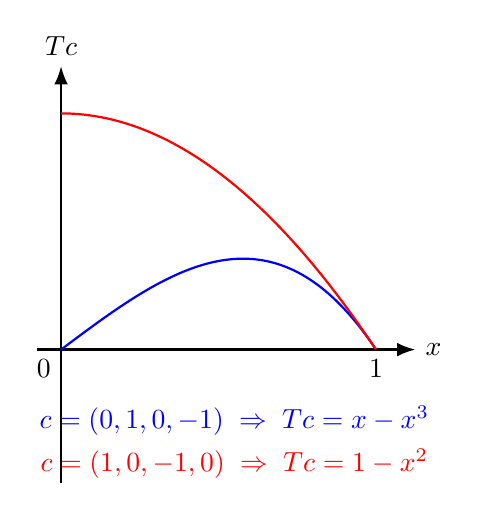
\begin{tikzpicture}[>=Latex, thick]
    % Axes: x in [0,1] scaled by 4, values scaled by 3
    \draw[->] (-0.3,0) -- (4.5,0) node[right] {$x$};
    \draw[->] (0,-1.7) -- (0,3.6) node[above] {$Tc$};

    % c = (0, 1, 0, -1):  Tc = x - x^3
    \draw[blue, thick] plot[domain=0:1, samples=60, smooth] ({4*\x}, {3*(\x - \x*\x*\x)});

    % c = (1, 0, -1, 0):  Tc = 1 - x^2
    \draw[red, thick] plot[domain=0:1, samples=60, smooth] ({4*\x}, {3*(1 - \x*\x)});

    % Endpoints
    \node[below left] at (0,0) {$0$};
    \node[below] at (4,0) {$1$};

    % Legend
    \node[blue] at (2.2, -0.9) {$c = (0, 1, 0, -1) \;\Rightarrow\; Tc = x - x^3$};
    \node[red]  at (2.2, -1.45) {$c = (1, 0, -1, 0) \;\Rightarrow\; Tc = 1 - x^2$};
\end{tikzpicture}
\end{center}
\end{example}

\begin{definition}[Linear functional]
\label{def:linear-functional}
A linear functional on $V$ is a linear operator whose target vector space is the
scalars themselves, $\mathbb{C}$ (or $\mathbb{R}$):
$$l : V \rightarrow \mathbb{C}, \qquad l(\alpha u + \beta v) = \alpha\, l(u) + \beta\, l(v).$$
\end{definition}
Examples of linear functionals:
\begin{itemize}
    \item On $\mathbb{C}^n$: $l(x) = \sum_{j=1}^{n} a_j x_j$ for a fixed vector
    $a \in \mathbb{C}^n$; e.g.\ $l(x) = x_1 + 2x_3$.
    \item The most important example: for a fixed $y \in V$,
    $$l(v) = \langle v, y \rangle$$
    is a linear functional, because the inner product is linear in its first slot.
    On $L^2(0, 1)$ this reads $l(f) = \int_0^1 f(t)\overline{g(t)}\dd t$ for a fixed
    $g \in L^2(0, 1)$.
    \item Special case on $L^2(0, 1)$ with $g = 1$: $l(f) = \int_0^1 f(t)\dd t$, the
    average value of $f$ -- its constant (``DC'') Fourier coefficient.
\end{itemize}
\begin{remark}
Not every linear functional is visibly an inner product, but on the spaces we care
about (Hilbert spaces) every bounded linear functional has this form: $l(v) =
\langle v, y\rangle$ for a unique $y \in V$. This fact is the Riesz representation
theorem.
\end{remark}
\begin{definition}[Dual Space]
\label{def:dual-space}
The space of all linear functionals on $V$ is itself a vector space, called the
\emph{dual space} of $V$:
$$V^{*} = \{l : V \rightarrow \mathbb{C} : l \text{ linear}\}, \qquad
(\alpha l + \beta m)(v) = \alpha\, l(v) + \beta\, m(v).$$
\end{definition}
\par Why is $V^{*}$ a vector space? The pointwise operations inherit every axiom
from the scalars; for instance additivity,
$$(\alpha l + \beta m)(u + v) = \alpha\, l(u+v) + \beta\, m(u+v) =
(\alpha l + \beta m)(u) + (\alpha l + \beta m)(v),$$
and the zero functional $l(v) \equiv 0$ is the additive identity.
\par On $\mathbb{C}^n$ the dual space is $n$-dimensional: every functional is
$l(x) = \sum_{j=1}^{n} a_j x_j$, a combination of the coordinate functionals
$l_j(x) = x_j$. In a Hilbert space the same thing happens through the inner
product: by the Riesz remark above, $y \mapsto \langle \cdot, y\rangle$ matches
each $y \in V$ with a distinct functional and exhausts all of (bounded) $V^{*}$ --
so the dual space is a copy of $V$ itself.

\begin{definition}[Convolution]
\label{def:convolution}
The convolution of $g$ and $f$ is
$$(g * f)(x) = \int_{-\infty}^{\infty} g(x - y)\, f(y)\dd y$$
This is an integral operator as above, with kernel $G(x, y) = g(x - y)$.
\end{definition}
Find the solution of the boundary value problem
\[
\begin{cases}
-u''(x)=f(x), & 0<x<1,\\
u(0)=0,\\
u(1)=0.
\end{cases}
\]

Show that the solution can be written in the form
\[
u(x)=\int_0^1 G(x,y)f(y)\,dy,
\]
where $G(x,y)$ is the Green's function for the differential operator
\[
L=-\frac{d^2}{dx^2}
\]
with the boundary conditions
\[
G(0,y)=G(1,y)=0.
\]

Derive the Green's function $G(x,y)$.
\begin{center}
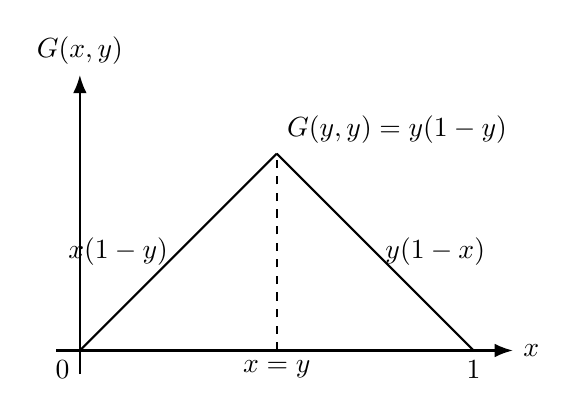
\begin{tikzpicture}[
    >=Latex,
    thick
]

% Axes
\draw[->] (-0.3,0) -- (5.5,0) node[right] {$x$};
\draw[->] (0,-0.3) -- (0,3.5) node[above] {$G(x,y)$};

% Green's function
\draw (0,0) -- (2.5,2.5);
\draw (2.5,2.5) -- (5,0);

% Dashed line at x = y
\draw[dashed] (2.5,0) -- (2.5,2.5);

% Labels
\node[below] at (2.5,0) {$x=y$};
\node[left] at (1.25,1.25) {$x(1-y)$};
\node[right] at (3.75,1.25) {$y(1-x)$};

% Endpoints
\node[below left] at (0,0) {$0$};
\node[below] at (5,0) {$1$};

% Peak
\node[above right] at (2.5,2.5) {$G(y,y)=y(1-y)$};

\end{tikzpicture}
\end{center}

\[
G(x,y)
=
\begin{cases}
x(1-y), & 0\leq x\leq y,\\[4pt]
y(1-x), & y\leq x\leq 1.
\end{cases}
\]
\begin{definition}[kernel]
\label{def:label} 
The kernel $\ker(G) = $ the null space of $G$ also written as $N(G)$ its nullspace 
\end{definition}

\section{Topics to review}
\label{sec:review-topics}
Green's functions and the continuous ($L^2$) applications of vector spaces are the
parts of this lecture that still need work. When going back over these notes,
review in this order.

\subsection*{Green's function material}
\begin{itemize}
    \item \textbf{The problem being solved:} $-u''(x) = f(x)$ on $0 < x < 1$ with
    $u(0) = u(1) = 0$ -- why it is reasonable to look for a solution of the form
    $u(x) = \int_0^1 G(x, y)f(y)\dd y$ at all.
    \item \textbf{Deriving $G(x,y)$:} away from $x = y$ the equation is
    $-G''(\cdot, y) = 0$, so $G$ is linear in $x$ on each side. The two conditions
    that pin it down are \emph{continuity} at $x = y$ (where $G(y,y) = y(1-y)$) and
    the \emph{jump condition} on the derivative,
    $$G_x(y^+, y) - G_x(y^-, y) = -1,$$
    which comes from integrating $-u'' = f$ across $x = y$. Re-derive the piecewise
    formula ($x(1-y)$ for $x \le y$, $y(1-x)$ for $y \le x$) from just these two
    conditions plus $G(0, y) = G(1, y) = 0$.
    \item \textbf{Verifying the solution:} differentiate
    $u(x) = \int_0^1 G(x,y)f(y)\dd y$ under the integral separately on $x < y$ and
    $x > y$, and see exactly where the jump in $G_x$ produces $u'' = -f$; then
    check $u(0) = u(1) = 0$ directly.
    \item \textbf{Kernel viewpoint:} $G$ is the kernel of an integral operator
    $Gf(x) = \int_0^1 G(x,y)f(y)\dd y$ on $L^2(0,1)$ -- compare with the
    convolution kernel $G(x, y) = g(x-y)$ in the Convolution definition above.
\end{itemize}

\subsection*{Continuous vector spaces and operators on them}
\begin{itemize}
    \item \textbf{Functions as vectors:} $L^2(0,1)$ as the infinite-dimensional
    analogue of $\mathbb{C}^n$ -- vectors are functions, inner products are
    integrals, and convergence in $L^2$ is \emph{neither} pointwise \emph{nor}
    uniform convergence in general (B\&N \S0.3.2; the single most important nuance
    for the rest of the course).
    \item \textbf{Finite-dimensional subspaces inside $L^2$:} the polynomial
    example ($T : \mathbb{C}^4 \rightarrow L^2(0,1)$ with range $P_3$); how
    orthogonal complements and projections (\S0.5.2) will let us decompose
    functions the way we decompose vectors.
    \item \textbf{Linear operators on function spaces:} the matrix example versus
    the integral operator example (\S0.6.1) -- what it takes for
    $Gf(x) = \int_a^b G(x, y) f(y) \dd y$ to be a well-defined map of $L^2$ into
    itself.
    \item \textbf{Functionals and the dual space:} functionals are operators with
    scalar output; the inner product functionals $v \mapsto \langle v, y\rangle$,
    and (Riesz) why on Hilbert spaces they exhaust the bounded dual.
    \item \textbf{Convolution:} $(g * f)(x) = \int g(x - y) f(y) \dd y$ as the
    integral operator whose kernel depends only on the difference $x - y$; it
    returns as the main character of the Fourier transform chapter (B\&N
    \S2.2.2, p.\ 107).
\end{itemize}

\subsection*{Textbook anchors and extra problems for this review}
\begin{itemize}
    \item Read: B\&N \S0.3 (especially \S0.3.2, convergence in $L^2$ versus
    uniform), \S0.5.2 (orthogonal complements/projections), \S0.6.1 (linear
    operators). Adjoints (\S0.6.2) are the likely next lecture.
    \item Chapter 0 exercises (pp.\ 34--38) beyond the homework: \#2 (verify the
    $l^2$ and $L^2$ inner products of Examples 0.2--0.3), \#4 ($L^2$ inner-product
    axioms, including positivity via continuity), \#5 (inner product on $l^2$),
    and especially \#6, \#7, \#8 -- sequences that converge in $L^2$ but not
    uniformly or pointwise.
\end{itemize}

\end{document}
